\documentclass{standalone}
\usepackage{tikz}
  \usetikzlibrary{positioning}
  \usetikzlibrary{arrows.meta}
  \usetikzlibrary{arrows, shapes, trees, positioning, decorations.markings, patterns}
  \usetikzlibrary{backgrounds}
  \usetikzlibrary[topaths]
  \usetikzlibrary{calc}
  \usetikzlibrary{backgrounds,fit,decorations.pathreplacing}
  \usetikzlibrary{shapes.multipart}
\usepackage{fontspec}
  \setmainfont[Ligatures=TeX]{Nimbus Roman No9 L}

\newcount\mycount

\usepackage{graphicx}
\graphicspath{{}{./assets/}}

\begin{document}
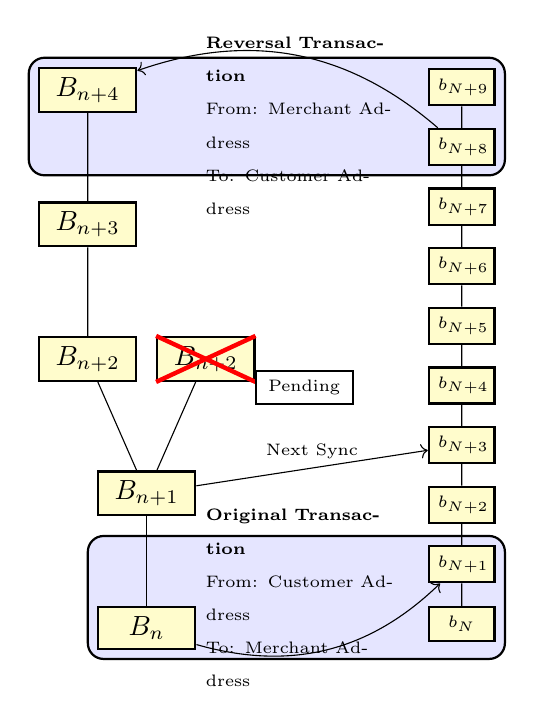
\begin{tikzpicture}[
% Gates and symbols style
   % and/.style={and gate US,thick,draw,fill=red!60,rotate=90,
	% 	anchor=east,xshift=-1mm},
    % or/.style={or gate US,thick,draw,fill=blue!60,rotate=90,
	% 	anchor=east,xshift=-1mm},
    % be/.style={circle,thick,draw,fill=green!60,anchor=north,
	% 	minimum width=0.7cm},
    % tr/.style={buffer gate US,thick,draw,fill=purple!60,rotate=90,
	% 	anchor=east,minimum width=0.8cm},
% Label style
    % label distance=3mm,
    level distance=2cm,
    every label/.style={blue},
% Event style
    event/.style={rectangle,thick,draw,grow=up,fill=yellow!20,text width=1cm,
		text centered,font=\sffamily,anchor=north},
    event2/.style={rectangle,thick,draw,grow=up,fill=yellow!20,text width=0.6cm,
		text centered,font=\sffamily,anchor=north,font={\fontsize{6pt}{12}\selectfont},
		level distance=1cm},
    font={\fontsize{9pt}{12}\selectfont}
% Children and edges style
    % edge from parent/.style={very thick,draw=black!70},
    % edge from parent path={(\tikzparentnode.south) -- ++(0,-1.05cm)
	% 		-| (\tikzchildnode.north)},
    % level 1/.style={sibling distance=7cm,level distance=1.4cm,
	% 		growth parent anchor=south,nodes=event},
    % level 2/.style={sibling distance=7cm},
    % level 3/.style={sibling distance=6cm},
    % level 4/.style={sibling distance=3cm}
%%  For compatability with PGF CVS add the absolute option:
%   absolute
    ]
  \tikzstyle{surround} = [fill=blue!10,thick,draw=black,rounded corners=2mm]

  % \draw [thick, gray, dotted, shift={(0.25,0.25)}] (-2, -1) grid [xstep=0,ystep=1.25] (7, 5.5);
  \node (s0) [event] {$B_n$} [grow=up]
    child {
      node (s1) [event] {$B_{n+1}$}
      child {
	node (s12) [event] {$B_{n+2}$}
      }
      child {
	node (s22) [event] {$B_{n+2}$}
	child {
	  node (s3) [event] {$B_{n+3}$}
	  child {
	    node (s41) [event] {$B_{n+4}$}
	  }
	}
      }
    };

  \node (b0) [event2] at (4,0) {$b_N$} [grow=up,level distance=1cm]
    child {
      node (b1) [event2] {$b_{N+1}$}
      child {
	node (b22) [event2] {$b_{N+2}$}
	child {
	  node (b3) [event2] {$b_{N+3}$}
	  child {
	    node (b41) [event2] {$b_{N+4}$}
	    child {
	      node (b5) [event2] {$b_{N+5}$}
	      child {
		node (b6) [event2] {$b_{N+6}$}
		child {
		  node (b7) [event2] {$b_{N+7}$}
		  child {
		    node (b8) [event2] {$b_{N+8}$}
		    child {
		      node (b9) [event2] {$b_{N+9}$}
		    }
		  }
		}
	      }
	    }
	  }
	}
      }
    };

  \draw[->] (s0) edge[bend right, below] node{} (b1);
  \draw[->] (b8) edge[bend right, above] node{} (s41);
\draw[red,ultra thick] (s12.south west) -- ($(s12.north east)-(0pt,0pt)$);
\draw[red,ultra thick] ($(s12.north west)-(0pt,0pt)$) -- (s12.south east);
  \node (p) [event,fill=white,font={\fontsize{6pt}{12}\selectfont}] at (2, 3) {Pending};
  \draw[->] (s1) edge[above,font={\fontsize{6pt}{12}\selectfont}] node{Next Sync} (b3);

  \node at (2, 6.1) [text width=2.5cm,font={\fontsize{6pt}{12}\selectfont}] {\textbf{Reversal Transaction} \\ From: Merchant Address \\ To: Customer Address};
  \node at (2, 0.1) [text width=2.5cm,font={\fontsize{6pt}{12}\selectfont}] {\textbf{Original Transaction} \\ From: Customer Address \\ To: Merchant Address};

  % \node (c2) at (5, 2.1) {Voting $V_{n+2}$};
  % \node (c4) at (5, 4.5) {Voting $V_{n+4}$};
% \node (v1) [rectangle,fill=black!40,minimum width=3cm] at (0, 2.2) {44444};

\begin{pgfonlayer}{background} 
  \node[surround] (background) [fit = (s41) (b8)] {};
\end{pgfonlayer}
\begin{pgfonlayer}{background} 
  \node[surround] (background) [fit = (s0) (b1)] {};
\end{pgfonlayer}

\end{tikzpicture}
\end{document}
